\documentclass[usenames,dvipsnames,aspectratio=169]{beamer}
\usepackage{../common/prg}

\title[1. előadás]{Programozás}
\subtitle{(GKxB\_INTM114)}

\begin{document}

%1
\begin{frame}[plain]
  \titlepage
  \logoalul
\end{frame}

\section{Bevezetés}
\subsection{Informatikai rendszerek fejlesztése}

%2
\begin{frame}
  \begin{itemize}
    \item Rendszertervezés (System Engineering)
    \begin{itemize}
      \item Üzleti folyamat tervezés (Business Process Engineering)
      \item Terméktervezés (Product Engineering)
    \end{itemize}
    \item Szoftvertervezés (Software Engineering)
    \begin{itemize}
      \item Követelményspecifikáció, -elemzés
      \item Tervezés
      \item \kiemel{Implementáció}
      \item Validáció, tesztelés
      \item Telepítés
      \item (Karbantartás, követés, továbbfejlesztés)
    \end{itemize}
  \end{itemize}
  \vfill
  \tiny{Irodalom: \hiv{\href{https://dtk.tankonyvtar.hu/xmlui/bitstream/handle/123456789/3684/2011-0042_szoftverfejlesztesi_folyamatok_magyar.pdf}{Dr. Ulbert Zsolt: Szoftverfejlesztési folyamatok és szoftver minőségbiztosítás} } }
\end{frame}

\subsection{Programozási nyelvek}

%3
\begin{frame}[fragile]
  \begin{itemize}
    \item Gépi kód
    \item Assembly
  \end{itemize}
  \begin{exampleblock}{pelda02.asm (Forrás: Agárdi Gábor: Gyakorlati Assembly)}
    \lstset{
      language=[x86masm]Assembler,
      keywordstyle=\color{black}\bfseries\underbar, % underlined bold black keywords
      identifierstyle=,           % nothing happens
      commentstyle=\color{blue},  % blue comments
      stringstyle=\ttfamily,      % typewriter type for strings
      showstringspaces=false,     % no special string spaces
      inputencoding=utf8,
      extendedchars=true
    }
    \tiny
    \lstinputlisting{pelda02.asm}
  \end{exampleblock}
\end{frame}

%4
\begin{frame}
  \begin{itemize}
    \item C
    \begin{itemize}
      \item Dennis Ritchie, Bell Laboratories (1969-1973): C programnyelv $\rightarrow$ UNIX operációs rendszer
      \item ``Szabványok'': K\&R (1978), ANSI (vagy C89, 1989), C99, C11.
      \item Tulajdonságok: általános célú, imperatív (parancsoló, a programnak \emph{hogyan} kell működnie a megfelelő 
állapotváltozások eléréséhez), strukturált (forrásfájlok, blokkok, ciklusok, stb. $\rightarrow$ áttekinthetőség)   
    \end{itemize}
    \item C++
    \begin{itemize}
      \item Bjarne Stroustroup (1979): ``C with Classes''
      \item ``Szabványok'': C++ (1983), ``The C++ Programming Language'' (1985), \dots, \hiv{\href{https://www.iso.org/standard/83626.html}{ISO/IEC 14882:2024 (C++23)}}
      \item Tulajdonságok: általános célú, procedurális, funkcionális, objektum-orientált, nagyrészt C kompatibilis
    \end{itemize}
  \end{itemize}
\end{frame}

%5
\begin{frame}
  \begin{itemize}
    \item Irodalom
    \begin{itemize}
      \item \hiv{\href{https://bookline.hu/product/home.action?_v=_&id=2371&type=22}{Brian W. Kernighan, Dennis M. Rithcie: A C 
programozási nyelv - Az ANSI szerint szabványosított változat}}
      \item \hiv{\href{https://www.libri.hu/konyv/benko_laszlo.programozzunk-c-nyelven-1.html}{Benkő László, Benkő Tiborné, Tóth 
Bertalan: Programozzunk C nyelven! - Kezdőknek - középhaladóknak}}
      \item Bauer Péter: C programozás
      \item \hiv{\href{http://jegyzet.sze.hu/}{Bauer Péter, Hatwágner F. Miklós: Programozás I-II}}
      \item \hiv{\href{https://www.libri.hu/konyv/bjarne_stroustrup.a-c-programozasi-nyelv-i-ii-kotet.html}
        {Bjarne Stroustrup: A C++ programozási nyelv I-II. kötet}}
        \item \hiv{\href{https://panem.hu/tantusz-konyvek/1473-c-.html}{Stephen R. Davis: C++ (Tantusz könyvek)}}
    \end{itemize}
    \item Szoftverek
    \begin{itemize}
      \item \hiv{\href{https://visualstudio.microsoft.com/vs/community/}{Microsoft Visual Studio}}
      \item \hiv{\href{https://www.qt.io/qt-features-libraries-apis-tools-and-ide/\#ide}{QT Creator IDE}}
      \item \hiv{\href{https://gcc.gnu.org/}{GNU Compiler Collection}}
      \item \hiv{\href{http://www.codeblocks.org/}{Code::Blocks}}
      \item \hiv{\href{https://www.geany.org/}{Geany}}
      \item \hiv{\href{https://www.onlinegdb.com}{OnlineGDB}}
    \end{itemize}
  \end{itemize}
\end{frame}

%6
\begin{frame}
  \begin{center}
    \includegraphics[width=1.0\textwidth,keepaspectratio=true]{./tiobe.png} \\
    \hiv{\href{https://www.tiobe.com/tiobe-index/}{Tiobe}} programozási nyelv népszerűségi index, 2025. február
  \end{center}
\end{frame}

%7
\begin{frame}
  \begin{columns}[T]
    \column{0.4\textwidth}
      \begin{exampleblock}{\textattachfile{szamok.cpp}{szamok.cpp}}
        \tiny
        \lstinputlisting[style=cpp]{szamok.cpp}
      \end{exampleblock}
    \column{0.6\textwidth}
      \begin{exampleblock}{\textattachfile{Szamok.java}{Szamok.java}}
        \tiny
        \lstset{
          language=Java,
          showstringspaces=false,
          keywordstyle=\color{MidnightBlue}\bfseries,
          stringstyle=\color{DarkOrchid},
          commentstyle=\color{Brown}}
        \lstinputlisting{Szamok.java}
      \end{exampleblock}
  \end{columns}
  \begin{columns}[T]
  \column{0.4\textwidth}
      \begin{exampleblock}{\textattachfile{szamok.php}{szamok.php}}
        \tiny
        \lstset{
          language=PHP,
          showstringspaces=false,
          keywordstyle=\color{MidnightBlue}\bfseries,
          stringstyle=\color{DarkOrchid},
          commentstyle=\color{Brown}}
        \lstinputlisting{szamok.php}
      \end{exampleblock}
    \column{0.6\textwidth}
      \begin{exampleblock}{\textattachfile{szamok.js}{szamok.js}}
        \tiny
        \lstset{
          language=Java,
          morekeywords={typeof, new, true, false, catch, function, return, null, catch, switch, var, if, in, while, do, else, 
case, break},
          showstringspaces=false,
          keywordstyle=\color{MidnightBlue}\bfseries,
          stringstyle=\color{DarkOrchid},
          commentstyle=\color{Brown}}
        \lstinputlisting{szamok.js}
      \end{exampleblock}
  \end{columns}
\end{frame}

%8
\section{Az első C++ programunk}

\subsection{Forrásfájltól a futtatásig}

\begin{frame}
  \begin{enumerate}
      \item Forrásszöveg megszerkesztése (többnyire \kiemel{.cpp} kiterjesztés, ASCII szövegfájl)
    \end{enumerate}
    \begin{exampleblock}{\textattachfile{elso.cpp}{elso.cpp}}
      \footnotesize
      \lstinputlisting[style=cpp]{elso.cpp}
    \end{exampleblock}
\end{frame}

%9
\begin{frame}[fragile]
  \begin{enumerate}
    \setcounter{enumi}{1}
    \item Összeállítás (build)
      \begin{block}{}
        g++ -Wall -o elso elso.cpp
      \end{block}
    \item Futtatás
    \begin{block}{Linux terminál}
      \scriptsize
      \begin{verbatim}
wajzy@wajzy-notebook:~/Dokumentumok/gknb_intm114/ea01$ ./elso 
Ez az elso C++ programunk!
wajzy@wajzy-notebook:~/Dokumentumok/gknb_intm114/ea01$
\end{verbatim}
    \end{block}
  \end{enumerate}
\end{frame}

%10
\begin{frame}
  Az összeállítási folyamat résztevékenységei
  \begin{enumerate}
    \item Fordítás (compiler)
    \begin{center}
      \includegraphics{forditas.pdf}
    \end{center}
    \begin{block}{Fordítás (compile) GCC-vel}
      g++ -Wall -c elso.cpp
    \end{block}
    Üzenetek típusai:
    \begin{itemize}
      \item hibaüzenetek (error) $\rightarrow$ szintaktikai hiba, nem jön létre tárgymodul
      \item figyelmeztető üzenetek (warning) $\rightarrow$ figyelmeztetés gyanús megoldásra, javaslattétel, létrejön a 
tárgymodul (object file)
    \end{itemize}
  \end{enumerate}
\end{frame}

%11
\begin{frame}[fragile]
  Az összeállítási folyamat résztevékenységei
  \begin{enumerate}
    \setcounter{enumi}{1}
    \item Kapcsoló-szerkesztés (link)
    \begin{itemize}
      \item fv.-ek tárgykódja: statikus könyvtárakban (.lib, run-time library vagy standard library)
    \end{itemize}
    \begin{block}{}
      g++ -o elso elso.o
    \end{block}
    \begin{center}
      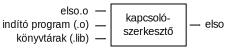
\includegraphics{kapcsszerk.pdf}
    \end{center}
    A kapcsoló-szerkesztő hibaüzenetei
  \end{enumerate}
\end{frame}

%12
\begin{frame}
  \begin{center}
    
\includegraphics[width=\textwidth]{folyamat.pdf}
  \end{center}
\end{frame}

%13
\subsection{A forrásfájl elemei}

\begin{frame}
  \begin{exampleblock}{\textattachfile{elso.cpp}{elso.cpp}}
    \footnotesize
    \lstinputlisting[style=cpp]{elso.cpp}
  \end{exampleblock}
\end{frame}

%14
\begin{frame}
  Megjegyzések:
  \begin{itemize}
    \item \kiemel{//} után a sor végéig
    \item \kiemel{/*} és \kiemel{*/} között akár több soron át
    \item Az előfeldolgozó törli őket
  \end{itemize}
  Direktívák:
  \begin{itemize}
    \item \kiemel{\#} kezdetű sorok
    \item \kiemel{\#include<\dots>} beszerkeszti a fejfájl (header) tartalmát $\rightarrow$ pl. konstansok, könyvtári 
függvények használatához (pl. \texttt{/usr/include/c++/4.8.4/iostream})
  \end{itemize}
  Direktíva, megjegyzés: előfeldolgozó (preprocessor) dolgozza fel
  \begin{center}
    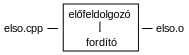
\includegraphics{elofeld.pdf}
  \end{center}
\end{frame}

%15
\begin{frame}
  A \texttt{\kiemel{main}} függvény
  \begin{itemize}
    \item Függvény: adatok és végrehajtható utasítások csoportja. Működésük paraméterekkel hangolható, értéket adhatnak vissza.
    \item Függvény definíció: teljes információt szolgáltat a függvényről
    \item \emph{típus függvénynév(formális-paraméterlista) \{ függvény-test \}}
    \item A \texttt{main} speciális: a program \kiemel{belépési pont}ja (entry point)
    \item Állapotkódot ad vissza az OS-nek (0: minden OK)
    \item Visszatérési érték: \texttt{\kiemel{return}} után
  \end{itemize}
  \kiemel{;} utasítás (statement) végének jelzése
\end{frame}

%16
\begin{frame}
  Szabványos folyamok
  \begin{itemize}
    \item Kimenet (stdout, $\approx$ képernyő), használata \texttt{\kiemel{cout}}-tal
    \item Bemenet (stdin, $\approx$ billentyűzet), használata \texttt{cin}-nel
    \item Hiba (stderr, $\approx$ képernyő), használata \texttt{cerr}-rel (nem pufferelt)
  \end{itemize}
  A \texttt{cout}
  \begin{itemize}
    \item üzenetek megjelenítése
    \item \texttt{\kiemel{{<}<}} operátor (műveleti jel): adat folyamba írása
    \item \texttt{\kiemel{endl}} újsor karakter + puffer ürítése
    \item Képernyőre íráskor valójában \emph{függvényhívás} történik
  \end{itemize}
\end{frame}

%17
\begin{frame}
  Névtér: halmaz, melyben minden azonosító egyedi
  \tiny
  \begin{exampleblock}{elso.cpp}
      \lstinputlisting[style=cpp]{elso.cpp}
  \end{exampleblock}
  \begin{exampleblock}{\textattachfile{elso_nevter.cpp}{elso\_nevter.cpp}}
      \lstinputlisting[style=cpp]{elso_nevter.cpp}
  \end{exampleblock}
\end{frame}

%18
\begin{frame}[fragile]
  \begin{block}{Átmeneti állományok megőrzése}
    g++ -save-temps -Wall -o "elso" "elso.cpp"
  \end{block}
  Fájlok: \textattachfile{elso.ii}{előfeldolgozás eredménye}, \textattachfile{elso.s}{assembly}.
  \vfill
  Feladat: írjuk ki az első 10 természetes szám négyzetét!
\end{frame}

%19
\section{Négyzetszámok}
\subsection{Literálok, aritmetikai operátorok}

\begin{frame}
  \footnotesize
  \begin{exampleblock}{\textattachfile{negyzetszamok.cpp}{negyzetszamok.cpp}}
      \vspace{-.3cm}
      \lstinputlisting[style=cpp]{negyzetszamok.cpp}
      \vspace{-.3cm}
  \end{exampleblock}
\end{frame}

%20
\begin{frame}[fragile]
  \footnotesize
  \begin{block}{Kimenet}
    \vspace{-.3cm}
    \begin{verbatim}
Termeszetes szamok negyzetei

1       1
2       4
3       9
4       16
5       25
6       36
7       49
8       64
9       81
10      100
    \end{verbatim}
    \vspace{-.5cm}
  \end{block}
\end{frame}

%21
\begin{frame}[fragile]
  \small
  Literálok: forrásszövegbe gépelt konstansok
  \footnotesize
  \begin{itemize}
    \item Egész konstansok
    \item Karakter konstansok: \kiemel{'}-ok között
    \item Karakterlánc (string) konstansok: \kiemel{"}-ek között
  \end{itemize}
  \small
  Vezérlőkarakterek, nem nyomtatható jelek, szintaktikai jelentéssel bíró jelek megadása $\rightarrow$ escape jelsorozat 
(escape sequence), \kiemel{\textbackslash} jel vezeti be, leggyakrabban használtak:
  \footnotesize
  \begin{center}
    \begin{tabular}{ll}
      Esc. szekv. & Jelentés\\ \hline
      \textbackslash{b} & visszalépés (backspace)\\
      \textbackslash{n} & új sor (new line)\\
      \textbackslash{r} & kocsi vissza (carriage return)\\
      \textbackslash{t} & vízszintes tabulátor (horizontal tab, HTAB)\\
      \textbackslash{\textbackslash} & fordított törtvonal (backslash)\\
      \textbackslash{'} & aposztróf\\
      \textbackslash{"} & idézőjel\\
      \textbackslash{ooo} & oktális szám\\
      \textbackslash{xhh} & hexadecimális szám\\
      \textbackslash{0} & zérus ASCII kódú karakter
    \end{tabular}
  \end{center}
\end{frame}

%22
\begin{frame}[fragile]
  Néhány aritmetikai operátor\\
  \begin{center}
    \begin{tabular}{lll}
      Operátor & Leírás & Példa\\ \hline
      \texttt{+} & Összeadás & $5 + 3 == 8$ \\
      \texttt{-} & Kivonás & $5 - 3 == 2$ \\
      \texttt{*} & Szorzás & $5 * 3 == 15$ \\
      \texttt{/} & Egészosztás & $5 / 3 == 1$ \\
      \texttt{\%} & Maradék képzés & $5 \% 3 == 2$ \\
    \end{tabular}
  \end{center}
  Megjegyzések:
  \begin{itemize}
    \item Kis egész kitevőjű hatványok $\rightarrow$ szorzás(ok)
    \item Meddig tart majd a gépelés (+kódméret nő, +hibalehetőségek), ha az első 1000 szám négyzetére lesz szükség?!
  \end{itemize}
\end{frame}

%23
\subsection{Változók, hozzárendelés és relációs operátorok, elöltesztelő ciklus}

\begin{frame}
  \begin{exampleblock}{\textattachfile{negyzetszamok2.cpp}{negyzetszamok2.cpp}}
    \vspace{-.2cm}
    \lstinputlisting[style=cpp]{negyzetszamok2.cpp}    
    \vspace{-.2cm}
  \end{exampleblock}
\end{frame}

%24
\begin{frame}
  Változók
  \begin{itemize}
    \item Pl.: \texttt{int szam;}
    \item típus
    \begin{itemize}
      \item az adat jellege (numerikus, szöveges)
      \item hogyan tárolják a memóriában
      \item milyen művelet végezhető vele
    \end{itemize}
    \item memóriaterület
    \begin{itemize}
      \item értéket tárolja típusnak megfelelően
      \item lokális változók (\kiemel{\{} és \kiemel{\}} közötti blokkokban) kezdőértéke definiálatlan, ,,memóriaszemét''
    \end{itemize}
    \item név, vagy azonosító (funkcióra utaló, ,,beszédes elnevezés'')
  \end{itemize}
\end{frame}

%25
\begin{frame}
  Azonosítóképzési szabályok
  \begin{itemize}
    \item Első karakter: kis- vagy nagybetű, ill. \_
    \item További karakterek: u. a., és számjegyek
    \item Nem lehet kulcsszó vagy védett azonosító
    \item Kis- és nagybetűre érzékenyek
    \item Ajánlás: ne kezdődjön egy vagy két \_ karakterrel
    \item Szignifikáns karakterek száma
  \end{itemize}
  \begin{columns}[T]
    \column{.5\textwidth}
      \begin{alertblock}{Mi lehet a gond?}
        Gipsz Jakab\\
        66\_os\_ut\\
        Menő\_Manó\\
        auto
      \end{alertblock}
    \column{.5\textwidth}
      \begin{exampleblock}{OK}
        meno\_mano\\
        Meno\_Mano\\
        sokReszbolOsszeteve
      \end{exampleblock}
  \end{columns}
\end{frame}

%26
\begin{frame}
  \begin{columns}[c]
    \column{.4\textwidth}
      Fontosabb egész típusok (fixpontos ábrázolás) $\to$ alaptípus és típusmódosítók\\
      \smallskip
      \hiv{\href{https://en.cppreference.com/w/cpp/types/integer}{Rögzített méretű egész típusok}} (C++11)
    \column{.5\textwidth}
      \scriptsize
      \vspace{-.2cm}
      \begin{center}
        \begin{tabular}{ll}
          Típus & Leírás \\ \hline\hline
          \texttt{char} & Ált. előjeles, 8 bites egész \\ \hline
          \texttt{signed char} & Előjeles 8 bites egész \\ \hline
          \texttt{unsigned char} & Előjel nélküli, 8 bites egész \\ \hline
          \texttt{short} & \multirow{3}{*}{Előjeles rövid egész} \\
          \texttt{signed short} & \\
          \texttt{signed short int} & \\ \hline
          \texttt{unsigned short} & \multirow{2}{*}{Előjel nélküli rövid egész} \\
          \texttt{unsigned short int} & \\ \hline
          \texttt{signed} & \multirow{3}{*}{Előjeles egész} \\
          \texttt{int} & \\
          \texttt{signed int} & \\ \hline
          \texttt{unsigned} & \multirow{2}{*}{Előjel nélküli egész} \\
          \texttt{unsigned int} & \\ \hline
          \texttt{long} & \multirow{3}{*}{Előjeles hosszú egész} \\
          \texttt{signed long} & \\
          \texttt{signed long int} & \\ \hline
          \texttt{unsigned long} & \multirow{2}{*}{Előjel nélküli hosszú egész} \\
          \texttt{unsigned long int} & \\
        \end{tabular}
      \end{center}
  \end{columns}
\end{frame}

%27
\begin{frame}
  Megjegyzések:
  \begin{itemize}
    \item Típusmódosítók: \texttt{signed/unsigned}, \texttt{short/long}
    \item Egész literál ábrázolása: \texttt{int}
    \item \texttt{char} típus mérete: mindig 1 bájt, de a karakter literál \texttt{int}-ben!
    \item \texttt{char} típus előjel-kezelése: platformtól és fordítótól függ, de ált. előjeles és beállítható
    \item \texttt{1 == sizeof(char) <= sizeof(short) <= sizeof(int) <= sizeof(long) <= sizeof(long long)}, ahol \texttt{sizeof} 
a típus/változó méretét bájtban megadó operátor
  \end{itemize}
\end{frame}

%28
\begin{frame}
  Változó definíció
  \begin{itemize}
    \item Általános alak: \emph{típus azonosítólista;}
    \item Azonosító, típus megadása, memóriaterület foglalása
    \item Pl.: \kiemel{\texttt{int x; int i, j, k; unsigned int y;}}
  \end{itemize}
  \vfill
  Értékadás
  \begin{itemize}
    \item Operátor: \kiemel{=}
    \item \emph{balérték} \kiemel{=} \emph{jobbérték};
    \item kifejezés (expression): értéket állít elő konstansok, változók, műveletek (operátorok) segítségével
  \end{itemize}
\end{frame}

%29
\begin{frame}
  Relációs operátorok
  \begin{center}
    \begin{tabular}{ll}
      Operátor & Leírás \\ \hline
      \texttt{==} & egyenlő \\
      \texttt{!=} & nem egyenlő \\
      \texttt{<} & kisebb \\
      \texttt{<=} & kisebb, vagy egyenlő \\
      \texttt{>} & nagyobb \\
      \texttt{>=} & nagyobb, vagy egyenlő \\
    \end{tabular}
  \end{center}
\end{frame}

%30
\begin{frame}
  Elöltesztelő ciklus
  \vfill
  \begin{columns}[c]
    \column{0.5\textwidth}
      \hspace{0.15cm} 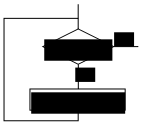
\includegraphics{eloltesztelo.pdf}
    \column{0.5\textwidth}
      \emph{{<}megelőző tevékenységek>}\\
      \emph{while(feltétel kifejezése) \{} \\
      \hspace{0.5cm} \emph{tevékenységek}\\
      \emph{\}}\\
      \emph{{<}további tevékenységek>}\\
  \end{columns}
  \vfill
  A \emph{ciklusmag} (ismételt rész) lehet
  \begin{itemize}
    \item egyetlen egyszerű utasítás
    \item összetett utasítás: több utasításból képzett blokk
  \end{itemize}
\end{frame}

%31
\section{Páros, páratlan}
\subsection{Feltételes vezérlési szerkezet}

\begin{frame}
  \small
  Olvassunk be egy egész számot, majd döntsük el, hogy páros-e!
  \begin{exampleblock}{\textattachfile{paros.cpp}{paros.cpp}}
    \footnotesize
    \vspace{-.2cm}
    \lstinputlisting[style=cpp]{paros.cpp}
    \vspace{-.2cm}
  \end{exampleblock}
\end{frame}

%32
\begin{frame}
  Beolvasás szabvány bemenetről: \kiemel{std::cin} \\
  \vfill
  Szelekció
  \vfill
  \begin{center}
    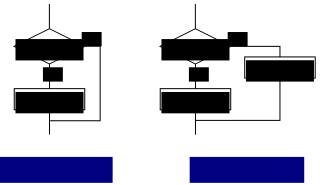
\includegraphics[width=.6\textwidth]{szelekcio.pdf}
  \end{center}
  \vfill
  Utasítások lehetnek összetettek $\rightarrow$ többirányú elágazás
\end{frame}

%33
\subsection{Műveletek precedenciája}

\begin{frame}
  Műveleti sorrend (kifejezések)
  \begin{itemize}
    \item zárójelezés
    \item műveletek precedenciája (időbeli sorrend)
  \end{itemize}
  \begin{center}
    \begin{tabular}{ll}
    Operátor & Asszociativitás\\ \hline
    sizeof & jobbról balra\\
    * / \% & balról jobbra\\
    + - & balról jobbra\\
    < <= > >= & balról jobbra\\
    == != & balról jobbra\\
    = & jobbról balra\\
    \end{tabular}
  \end{center}
  Vezérlési szerkezetek
  \begin{itemize}
    \item szekvencia
    \item iteráció
    \item szelekció
  \end{itemize}
\end{frame}

\end{document}
